\documentclass[11pt]{article}
\usepackage[margin=1in]{geometry}
\usepackage[T1]{fontenc}
\usepackage{lmodern}
\usepackage{amsmath,amssymb,amsthm,mathtools}
\usepackage{enumitem}
\usepackage{booktabs,tabularx,array}
\usepackage{graphicx}
\usepackage{caption}
\usepackage{float}
\usepackage{microtype}
\usepackage[dvipsnames]{xcolor}
\usepackage[colorlinks=true,linkcolor=MidnightBlue,citecolor=MidnightBlue,urlcolor=MidnightBlue]{hyperref}

\newtheorem{theorem}{Theorem}
\newtheorem{proposition}[theorem]{Proposition}
\newtheorem{lemma}[theorem]{Lemma}
\newtheorem{corollary}[theorem]{Corollary}
\theoremstyle{definition}
\newtheorem{definition}[theorem]{Definition}
\newtheorem{assumption}{Assumption}
\theoremstyle{remark}
\newtheorem{remark}[theorem]{Remark}

\newcommand{\E}{\mathbb{E}}
\newcommand{\KL}{\mathrm{KL}}
\newcommand{\Var}{\mathrm{Var}}
\newcommand{\pref}{\pi_{\mathrm{ref}}}
\newcommand{\sgn}{\operatorname{sgn}}
\newcommand{\osc}{\operatorname*{osc}}
\newcommand{\Dinf}{D_{\infty}}
\newcommand{\cY}{\mathcal{Y}}
\newcommand{\cL}{\mathcal{L}}
\newcommand{\1}{\mathbb{1}}
\newcommand{\rr}{R-REBEL}
\newcommand{\rrs}{R-REBEL-std}

\begin{document}
\begin{center}
{\LARGE Why Group Standardization Works in \rr{}}\\[6pt]
{\large A first-principles theory, with further results in the style of REBEL}\\[8pt]
{\small Working notes --- September 26, 2026}
\end{center}

\begin{abstract}
\rr{} fits pairwise differences of rewards with pairwise differences of policy
log-ratios under a robust discrepancy; its \emph{std} variant first divides the
rewards of each group by their in-group standard deviation. This note explains,
from first principles and in the notation of the draft~\cite{draft}, what that
single change does and why it matters for the constrained (Lagrangian) reward of
the multi-objective problem. In one sentence: \emph{plain \rr{} charges a fixed KL
price $\beta$ for moving away from the reference; standardization turns the price
into a fixed KL budget, the same in every context, and the Lagrangian reward is
exactly the case where a fixed price fails, because its scale changes by orders of
magnitude with the threshold $\tau$.}
Part~I makes this precise: the population target, the trust-region
interpretation, the normalized natural-gradient dynamics, and an exact
characterization of the finite-group target (a Gibbs policy on a bounded,
rank-preserving transform of the reward). Part~II follows the programme of the
REBEL paper~\cite{rebel} --- Gauss--Newton/NPG connection, preference extension,
convergence and agnostic regret guarantees --- and adds results specific to the
Lagrangian reward. The quantitative claims are also checked numerically on
small tabular problems (Appendix~\ref{app:checks}).
\end{abstract}

\begin{table}[H]
\centering\footnotesize
\renewcommand{\arraystretch}{1.15}
\begin{tabularx}{\textwidth}{@{}>{\raggedright\arraybackslash}p{4.3cm}>{\raggedright\arraybackslash}p{3.1cm}X@{}}
\toprule
 & plain \rr{} & \rrs{} \\
\midrule
window target, large $G$ & $\pref\, e^{r/\beta}$ & $\pref\, e^{r/(\beta\sigma_q(x))}$ \hfill Thm.~\ref{thm:target}\\
window target, finite $G$ ($\ell_2$) & $\pref\, e^{r/\beta}$ & $\pref\, e^{G\zeta_q/((G-1)\beta)}$, $\zeta_q$ bounded and rank-preserving \hfill Thm.~\ref{thm:finiteG}\\
invariant to & $r+b(x)$ & $a(x)\,r+b(x)$, any $a>0$ \hfill Cor.~\ref{cor:invariance}\\
per-window KL (small steps) & $\sigma(x)^2/(2\beta^2)$ & $1/(2\beta^2)$ \hfill Prop.~\ref{prop:budget}\\
largest per-window log-ratio change & $R(x)/\beta$ & $\le 2\sqrt{G}/\beta$ \hfill Cor.~\ref{cor:finiteG}\\
late-phase odds contraction per window & $e^{-\Delta/\beta}$ & $e^{-\sqrt{G}/\beta}$ \hfill Cor.~\ref{cor:finiteG}\\
weight of a context in the loss & $2\hat\sigma(x)^2$ & $2$ \hfill Prop.~\ref{prop:balance}\\
Gauss--Newton step, $\beta^2\delta^\top F\delta$ & $\|\Pi r_c\|^2$ & $R^2_{\mathrm{compat}}\le 1$ \hfill Prop.~\ref{prop:gn}\\
windows to relative accuracy $\varepsilon$ & grows with $R_{\max}/R(x)$ & independent of the reward scale \hfill Thm.~\ref{thm:rate}, Prop.~\ref{prop:separation}\\
surely-infeasible group, dependence on $\lambda$ & targets $\propto\lambda$ & none \hfill Prop.~\ref{prop:branch}\\
group size $G=2$ & REBEL & online IPO $=$ REBEL's self-play preference update \hfill Prop.~\ref{prop:G2}\\
\bottomrule
\end{tabularx}
\caption{What standardization changes. $\sigma$: reward standard deviation within a
context; $R(x)$: reward range of context $x$; $\Delta$: reward gap to the best
output; $\zeta_q$: expected in-group z-score (Definition~\ref{def:zeta}).}
\label{tab:summary}
\end{table}

\tableofcontents

%==============================================================================
\part{Core theory}
%==============================================================================

\section{Setting and notation}\label{sec:setting}

\paragraph{Contexts, outputs, rewards.} Throughout, $x$ denotes the \emph{full}
context. In the benchmark $x=(x_{\mathrm{text}},\tau)$ is the pair (input text,
threshold), written $\bar x$ on the slides~\cite{slides}. $y\in\cY$ is the output of
the policy (the prompt $z$, in prompt optimization); $\cY$ is finite (for instance,
all $L$-token strings). $r(x,y)$ is the reward, $\pi(y\mid x)$ the policy,
$\pref(y\mid x)$ the reference, $\beta>0$, and
\[
  h_\pi(x,y) \coloneqq \beta\log\frac{\pi(y\mid x)}{\pref(y\mid x)} .
\]

\paragraph{The loss.} Given a group $y_{1:G}$ drawn i.i.d.\ from a sampler
$q(\cdot\mid x)$ with rewards $r_i=r(x,y_i)$, the \rr{} loss of the draft (its
Eq.~(6)) with discrepancy $d(a,b)=\ell(b-a)$ is
\begin{equation}\label{eq:loss}
  \cL_\pi(x,y_{1:G}) = \frac{1}{G(G-1)}\sum_{i\neq j}
  \ell\bigl(h_\pi(x,y_i)-h_\pi(x,y_j)-(\tilde r_i-\tilde r_j)\bigr),
\end{equation}
where $\ell$ is even with $\ell(0)=0$ and $\ell(e)>0$ for $e\neq0$: $\ell_2(e)=e^2$,
$\ell_1(e)=|e|$, the Huber loss, and so on. Plain \rr{} uses $\tilde r_i=r_i$; \rrs{}
uses $\tilde r_i=r_i/\hat\sigma$ with $\hat\sigma^2=\frac{1}{G-1}\sum_i(r_i-\bar r)^2$.
Only differences enter, so the std variant regresses onto differences of the
in-group z-scores
\begin{equation}\label{eq:z}
  z_i \coloneqq \frac{r_i-\bar r}{\hat\sigma}\qquad(z_i\coloneqq 0\text{ if }\hat\sigma=0).
\end{equation}
For every non-flat group, $\sum_i z_i=0$ and $\sum_i z_i^2=G-1$.

\paragraph{Iterations.} As in REBEL's Algorithm~1, we analyse the idealized
iteration: at iteration $t$ the reference is the current policy, $\pref=\pi_t$;
groups are drawn from $q_t(\cdot\mid x)$ (the current policy, the draft's perturbed
samplers $\pi_{\epsilon_i}$, or a mixture with a base distribution $\mu$); and
$\pi_{t+1}$ minimizes $\E[\cL_\pi]$. One iteration is a \emph{window}. In the
implementation a window is a number of Adam steps against a lagged reference while
the sampler follows the moving policy; Section~\ref{sec:sampling} discusses what
changes.

\paragraph{The multi-objective reward.} On the slides,
\begin{equation}\label{eq:lagrangian}
  r(x,y)=\E_{o\sim\pi_{\mathrm{task}}(\cdot\mid y,x_{\mathrm{text}})}
  \bigl[s_1(o)\,\1\{s_2(o)\ge\tau\}+\lambda\,(s_2(o)-\tau)\,\1\{s_2(o)<\tau\}\bigr],
\end{equation}
with $s_1$ the sentiment score, $s_2$ the content score and $\lambda>0$ the
multiplier. Its scale depends on $\tau$ and on the policy. In a group that meets
the floor, $r$ spreads like the sentiment score, over tens of points on a
$0$--$100$ scale. In a group that misses it, $r$ spreads like $\lambda$ times the
content score, about a hundred times less at $\lambda=0.01$. Standardization is
aimed at exactly this heterogeneity.

%------------------------------------------------------------------------------
\section{What \rrs{} optimizes}\label{sec:target}

Repeat the draft's derivation (its Eqs.~(3)--(5)) with $r$ replaced by $r/\sigma$.
Because $\sigma$ depends only on the context, it passes through unchanged.

\begin{theorem}[Target of \rrs{}, large groups]\label{thm:target}
Let $q(\cdot\mid x)$ have full support and let $\sigma_q(x)>0$ be the standard
deviation of $r(x,y)$ for $y\sim q(\cdot\mid x)$. Replace $\hat\sigma$ by its
large-$G$ limit $\sigma_q(x)$. Then, for every discrepancy $\ell$ as above, the
population loss
\[
  \cL^\infty(\pi)=\E_x\,\E_{y,y'\sim q}\;
  \ell\Bigl(h_\pi(x,y)-h_\pi(x,y')-\frac{r(x,y)-r(x,y')}{\sigma_q(x)}\Bigr)
\]
is nonnegative, and it is zero if and only if, for almost every $x$,
\begin{equation}\label{eq:target}
  \pi(\cdot\mid x)=\pi^\star_{\mathrm{std}}(\cdot\mid x)\propto
  \pref(\cdot\mid x)\,\exp\Bigl(\frac{r(x,\cdot)}{\beta\,\sigma_q(x)}\Bigr).
\end{equation}
Equivalently, \rrs{} solves the KL-regularized problem of the draft (its Eq.~(1))
with a \emph{context-dependent temperature}:
\[
  \max_\pi\;\E_x\Bigl[\E_{y\sim\pi}r(x,y)-\beta\,\sigma_q(x)\,\KL\bigl(\pi(\cdot\mid x)\,\|\,\pref(\cdot\mid x)\bigr)\Bigr]
  =\max_\pi\;\E_x\Bigl[\E_{\pi}\Bigl[\frac{r}{\sigma_q(x)}\Bigr]-\beta\,\KL(\pi\,\|\,\pref)\Bigr].
\]
\end{theorem}

So std is plain \rr{} with $\beta$ replaced by $\beta_{\mathrm{eff}}(x)=\beta\,\sigma_q(x)$.
It is an adaptive KL coefficient, set per context and in closed form. RLHF
pipelines use a feedback controller for this job~\cite{ziegler}. The exact
finite-group statement is Theorem~\ref{thm:finiteG}.

\begin{corollary}[Invariance]\label{cor:invariance}
Replacing $r$ by $a(x)\,r+b(x)$ with $a(x)>0$ leaves every $z_i$ unchanged. Hence the
std loss~\eqref{eq:loss} is unchanged for every $\pi$ and every sample, even at
finite $G$. Plain \rr{} is invariant only to shifts $b(x)$.
\end{corollary}

The $\tau$-dependent scaling $r'=g(\tau)\,r$ of the slides (method~1 on the ``reward
modifications'' slide) is therefore a no-op under std. Standardization is the
data-driven choice $g=1/\sigma$, and it also adapts to $x$ and to the progress of
training.

%------------------------------------------------------------------------------
\section{A fixed KL budget}\label{sec:budget}

\begin{proposition}[Scale-free trust region]\label{prop:budget}
Take $q=\pref$, as holds at a reference refresh with on-policy sampling. Fix $x$ and
let $u=(r-\E_{\pref}r)/\sigma$ be the standardized reward, with cumulant generating
function $\Lambda(t)=\log\E_{\pref}e^{tu}$. Then
\[
  \KL(\pi^\star_{\mathrm{std}}\,\|\,\pref)=\tfrac1\beta\Lambda'(\tfrac1\beta)-\Lambda(\tfrac1\beta)\eqqcolon\varepsilon_\beta(x),
  \qquad
  \E_{\pi^\star_{\mathrm{std}}}r-\E_{\pref}r=\sigma\,\Lambda'(\tfrac1\beta).
\]
\begin{enumerate}[label=(\roman*),itemsep=1pt,topsep=2pt]
\item Both quantities depend on the context only through the \emph{shape} of the
law of $u$, never through the reward's scale or location.
\item $\varepsilon_\beta=\frac{1}{2\beta^2}+\frac{\gamma}{3\beta^3}+O(\beta^{-4})$
and the gain is $\sigma\bigl(\frac1\beta+\frac{\gamma}{2\beta^2}+O(\beta^{-3})\bigr)$,
where $\gamma=\E_{\pref}u^3$ is the skewness. For a Gaussian-shaped $u$ both are
exact: the KL is $1/(2\beta^2)$ and the gain is $\sigma/\beta$.
\item $\pi^\star_{\mathrm{std}}$ maximizes $\E_\pi r$ subject to
$\KL(\pi\,\|\,\pref)\le\varepsilon_\beta(x)$: each window is a \emph{trust-region}
step with a context-independent radius.
\item For plain \rr{}, $\KL(\pi^\star\,\|\,\pref)=\frac{\sigma}{\beta}\Lambda'(\frac{\sigma}{\beta})-\Lambda(\frac{\sigma}{\beta})
=\frac{\sigma^2}{2\beta^2}+O(\sigma^3/\beta^3)$, which is quadratic in the reward scale.
\end{enumerate}
\end{proposition}

With the Lagrangian reward~\eqref{eq:lagrangian}, a single $\beta$ is too small
for one branch or too large for the other. The per-window KL of plain \rr{} differs
by about $10^4$ between a group that meets the floor and one that does not
(spreads differing by $\sim\!100$). Either the high-$\tau$ contexts barely move or
the low-$\tau$ contexts collapse within one window. Standardization gives every
context the same budget.

%------------------------------------------------------------------------------
\section{Refreshing the reference: a normalized natural gradient}\label{sec:npg}

\begin{proposition}[Normalized mirror ascent]\label{prop:npg}
Suppose every window is solved exactly with on-policy sampling ($q_t=\pi_t$) and
large groups. Then
\begin{equation}\label{eq:md}
  \pi_{t+1}(y\mid x)\propto\pi_t(y\mid x)\exp\bigl(\eta_t(x)\,r(x,y)\bigr),
  \qquad \eta_t(x)=\frac{1}{\beta\,\sigma_{\pi_t}(x)} .
\end{equation}
\begin{enumerate}[label=(\roman*),itemsep=1pt,topsep=2pt]
\item This is mirror ascent on $J(\pi)=\E_\pi r$ with the KL mirror map~\cite{beck}, with a
per-context step $\eta_t(x)$.
\item With tabular logits, $\pi_\theta(y\mid x)\propto e^{\theta_{x,y}}$, the update is
$\theta_{t+1}=\theta_t+A_t/(\beta\sigma_t)$ with $A_t=r-J_t$. Here $A_t$ is the
natural gradient of $J$ at $\pi_t$~\cite{kakade}, and its Fisher norm is exactly
$\sigma_t$. Every window is therefore a natural-gradient step of Fisher length
exactly $1/\beta$: a \emph{normalized} natural policy gradient.
\item Unrolled, $\pi_t\propto\pi_0\,e^{T_t(x)\,r}$ with $T_t=\sum_{s<t}\eta_s$. Every
iterate is a Gibbs policy (full support), and as $T_t\to\infty$ the iterates
concentrate on $\arg\max_y r(x,y)$, the constrained optimum for that $(x_{\mathrm{text}},\tau)$.
\end{enumerate}
\end{proposition}

Two consequences follow. First, standardized progress does not stall as the policy
sharpens: $\sigma_t$ shrinks, so $\eta_t$ grows. Plain \rr{} has $\eta=1/\beta$, so its
progress per window is proportional to $\sigma_t$; it is tied to the reward's units
and dies out exactly as the policy approaches the optimum. Second, in this
large-group idealization $\eta_t$ is \emph{unbounded} as $\sigma_t\to0$.
Section~\ref{sec:finiteG} shows that finite groups cap it.

%------------------------------------------------------------------------------
\section{Finite groups, exactly}\label{sec:finiteG}

The algorithm divides by the in-group sample standard deviation $\hat\sigma$, which
is not merely a noisy copy of $\sigma$: it is computed from the same samples it
scales, so a large reward gap inflates its own denominator. For $\ell_2$ this has a
closed form.

\begin{definition}[Expected in-group z-score]\label{def:zeta}
For a sampler $q$ and group size $G$, let
$\zeta_q(x,y)\coloneqq\E\bigl[z_1\,\big|\,y_1=y\bigr]$, where $z_1$ is the in-group
z-score~\eqref{eq:z} of member~1 and the other $G-1$ members are drawn i.i.d.\ from
$q(\cdot\mid x)$.
\end{definition}

\begin{theorem}[Exact finite-group target]\label{thm:finiteG}
Let $\ell=\ell_2$, let every $\log\pi(y\mid x)$ be a free parameter (tabular), let
$q(\cdot\mid x)$ have full support, and let $G\ge2$. The expected loss $\E[\cL_\pi]$ has
the unique minimizer
\begin{equation}\label{eq:finiteG}
  \pi^+(y\mid x)\;\propto\;\pref(y\mid x)\,\exp\Bigl(\frac{G}{G-1}\,\frac{\zeta_q(x,y)}{\beta}\Bigr).
\end{equation}
The same holds with noisy rewards, with $\zeta_q$ then also averaging over the noise.
\end{theorem}

So the finite-group target is still a Gibbs policy, but on the \emph{transformed}
reward $\zeta_q$ and at temperature $\beta(G-1)/G$. The transform is explicit:

\begin{lemma}[The in-group z-score is an algebraic sigmoid]\label{lem:phi}
Fix the other $G-1$ members, with mean $m'$ and sum of squared deviations $V'$. A
member with reward $r$ has z-score
\[
  z=\varphi(r)=\frac{\sqrt{G-1}\;c\,t}{\sqrt{V'+c\,t^2}},\qquad t=r-m',\quad c=\frac{G-1}{G}.
\]
If $V'>0$, $\varphi$ is strictly increasing, with $\varphi'=\sqrt{G-1}\,c\,V'/(V'+ct^2)^{3/2}$;
if $V'=0$ it is the step $\frac{G-1}{\sqrt G}\sgn(t)$. It is linear for small $|t|$,
and $|\varphi|$ saturates at $(G-1)/\sqrt G$ (Samuelson's bound~\cite{samuelson}).
\end{lemma}

\begin{corollary}[Properties of the finite-group target]\label{cor:finiteG}
In the setting of Theorem~\ref{thm:finiteG}, with deterministic rewards for (a) and (d):
\begin{enumerate}[label=(\alph*),itemsep=1pt,topsep=2pt]
\item \emph{Ranking is preserved.} If $r(x,y)>r(x,y')$ then $\zeta_q(x,y)\ge\zeta_q(x,y')$,
strictly when the others' rewards are not almost surely all equal. Hence
$\arg\max_y\zeta_q=\arg\max_y r$ for every sampler.
\item \emph{A hard trust region.} $\osc_y\log\bigl(\pi^+(y\mid x)/\pref(y\mid x)\bigr)\le 2\sqrt G/\beta$.
Consequently $\Dinf(\pi^+\|\pref)\le2\sqrt G/\beta$, $\Dinf(\pref\|\pi^+)\le2\sqrt G/\beta$
and $\KL(\pi^+\|\pref)\le2\sqrt G/\beta$, for every sampler and every reward scale.
\item \emph{Bounded influence of extreme rewards.} An output whose reward lies far
from the rest receives a saturated target, not a proportional one.
\item \emph{Constant-speed late phase.} If $q\to\delta_{y^\star}$ (unique best output
$y^\star$), then $\frac{G}{G-1}(\zeta_q(y^\star)-\zeta_q(y))\to\sqrt G$ for every $y\neq y^\star$.
So once the policy concentrates, each window multiplies the odds of every
suboptimal output by $e^{-\sqrt G/\beta}$ ($e^{-8}$ at $G=16$, $\beta=\tfrac12$),
whatever its reward gap. Plain \rr{} uses $e^{-\Delta/\beta}$ (scale-dependent);
the large-$G$ limit uses $e^{-\Delta/(\beta\sigma_t)}\to0$ (no trust region at the end).
\item \emph{Large groups.} As $G\to\infty$, $\zeta_q\to(r-\E_qr)/\sigma_q$ and
$G/(G-1)\to1$, recovering Theorem~\ref{thm:target}.
\end{enumerate}
\end{corollary}

\begin{figure}[t]
\centering
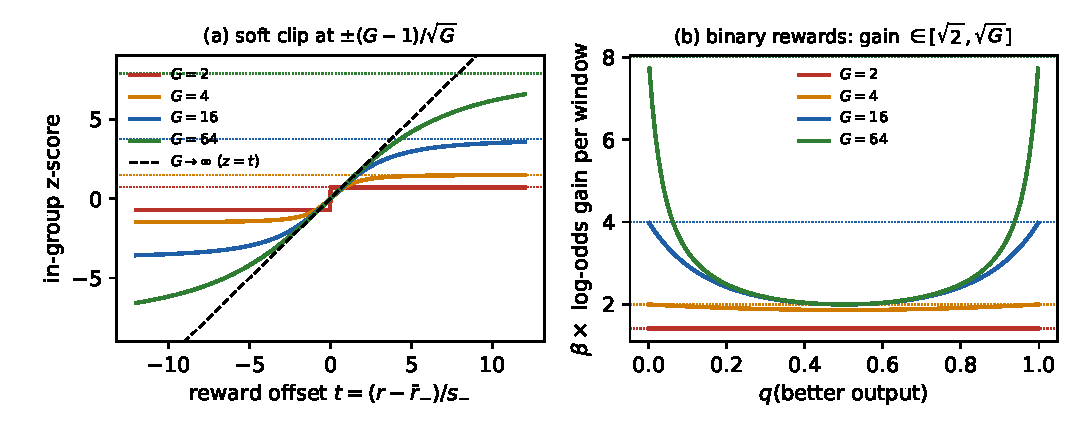
\includegraphics[width=\textwidth]{figures/squashing.pdf}
\caption{\textbf{(a)}~In-group z-score of one member as a function of its reward
offset $t$ from the other members' mean, in units of their sample standard
deviation $s_-$ (Lemma~\ref{lem:phi}, with $V'=(G-2)s_-^2$). $G=2$ keeps only the sign,
$G\to\infty$ is linear; in between, the z-score is the standardized reward softly
clipped at $\pm(G-1)/\sqrt G$ (dotted). \textbf{(b)}~Binary rewards:
$\beta\times$ the per-window log-odds gain of the better output as a function of its
current probability (Theorem~\ref{thm:finiteG}, $q=\pi_t$). It never depends on the
reward gap; it lies in $[2\sqrt{(G-1)/G},\sqrt G]$ and tends to $\sqrt G$ as the policy
concentrates (Corollary~\ref{cor:finiteG}(d)).}
\label{fig:squashing}
\end{figure}

%------------------------------------------------------------------------------
\section{Sampling: exploration and on-policy fixed points}\label{sec:sampling}

\begin{remark}[Refining the draft's Remark~1]\label{rem:sampler}
For plain \rr{}, the minimizer does not depend on the sampler (draft, Eqs.~(7) and~(9)).
For \rrs{} it does, because $\sigma_q$ (or $\zeta_q$) is measured under $q$. The sampler,
including the exploration perturbation, sets the temperature: \emph{how far} a
window moves. By Corollary~\ref{cor:finiteG}(a) it does not set the ranking, so the
iterates still head to the $\arg\max$. Exploration that adds low-reward samples
inflates $\hat\sigma$ and makes the on-policy part of the update more conservative.
\end{remark}

In the implementation the sampler is the moving policy itself. The target is then
self-referential, and the population picture breaks:

\begin{proposition}[On-policy, large groups: no fixed point for small $\beta$]\label{prop:nofp}
Take two outputs whose rewards differ by $\Delta>0$, uniform $\pref$, and let the
sampler be the current policy $\pi$ with $\sigma_\pi=\Delta\sqrt{p(1-p)}$, where $p=\pi(\text{better})$.
A self-consistent fixed point, $\pi\propto\pref\exp\bigl(r/(\beta\sigma_\pi)\bigr)$, exists if and only if
$\beta\ge\beta_c=\min_{s>0}\cosh(s)/s\approx1.509$. For $\beta<\beta_c$ the target
log-odds $2\cosh(\omega/2)/\beta$ exceeds the current log-odds $\omega$ for every $\omega$, so
the within-window regression drives $\pi$ to a point mass.
\end{proposition}

\begin{proposition}[On-policy, finite groups: a fixed point inside the trust region]\label{prop:fp}
For finite $G$ the map $q\mapsto\pref\exp\bigl(G\zeta_q/((G-1)\beta)\bigr)/Z_q$ has a
fixed point, and every fixed point satisfies Corollary~\ref{cor:finiteG}(b).
In the binary example at $G=16$, $\beta=\tfrac12$ the fixed point has log-odds
$7.99$, inside the bound $2\sqrt G/\beta=16$.
\end{proposition}

So finite group size is not an approximation error to be taken to infinity. It is
what keeps on-policy std a trust region.

%------------------------------------------------------------------------------
\section{Robust discrepancies under standardization}\label{sec:robust}

\begin{proposition}[First-order structure]\label{prop:firstorder}
Let $\psi=\ell'$. At a window start ($\pi=\pref$), over $S$ groups with $P=G(G-1)/2$
pairs each and the loss averaged over pairs,
\[
  \nabla_\theta\cL=-\frac{\beta}{SP}\sum_{\text{groups}}\sum_{i=1}^G u_i\,\nabla_\theta\log\pi(y_i),
  \qquad u_i=\sum_{j\neq i}\psi(z_i-z_j).
\]
For $\ell_2$, $u_i=2Gz_i$, which is $2G$ times GRPO's advantage. For $\ell_1$ (without ties),
$u_i=2\,\mathrm{rank}_i-(G+1)$, a centered rank: invariant to every increasing
transform of $r$ and equal to the fitness shaping of natural evolution
strategies~\cite{nes}. For Huber, $u_i=\sum_j\mathrm{clip}(z_i-z_j,-\delta,\delta)$.
\end{proposition}

For $\ell_1$, therefore, \emph{the rank sets the direction and standardization sets
the distance.} The first push is the same with or without std; std changes only
where the fit stops, which is the trust-region radius of
Proposition~\ref{prop:budget}. Standardization also supplies the scale that robust
M-estimation needs~\cite{huber}: Huber's $\delta$ and Cauchy's $c$ are measured in
residual units, and after standardization $\delta=1$ means ``one in-group standard
deviation'' in every context.

\begin{proposition}[Pairwise differencing symmetrizes noise]\label{prop:symm}
Let the observed rewards be $\hat r(y_i)=r(y_i)+\epsilon_i$, with the $\epsilon_i$
independent across members and either identically distributed (any shape) or each
symmetric about zero. Then $\epsilon_i-\epsilon_j$ is symmetric, and for every even,
convex $\ell$ and fixed $s>0$ the minimizer over $h$ of
$\E\,\ell\bigl(h-(\hat r_i-\hat r_j)/s\bigr)$ is $(r(y_i)-r(y_j))/s$. It is unique if
$\ell$ is strictly convex, or if $\ell=\ell_1$ and $\epsilon_i-\epsilon_j$ has positive
density at $0$.
\end{proposition}

\begin{lemma}[Bounded targets]\label{lem:bounded}
$|z_i|\le(G-1)/\sqrt G$ and $|z_i-z_j|\le\sqrt{2(G-1)}$, both tight. At $G=16$ every
regression target lies in $[-5.48,5.48]$, whatever the reward scale.
\end{lemma}

%------------------------------------------------------------------------------
\section{Balancing the \texorpdfstring{$\tau$}{tau}-conditioned network}\label{sec:balance}

\begin{proposition}[Every context gets the same weight]\label{prop:balance}
At a window start, the $\ell_2$ loss of a group, averaged over its pairs, equals
$2\hat\sigma^2$ for plain \rr{} and \emph{exactly} $2$ for \rrs{}, for every non-flat
group. For $\ell_1$ it is $\hat\sigma\,m$ versus $m$, where
$m=\overline{|z_i-z_j|}\in(0,\sqrt{2(G-1)}]$ depends only on the shape of the group's
rewards.
\end{proposition}

A shared, $\tau$-conditioned network trained without std weights each $(x,\tau)$ by
its reward variance. It spends its capacity on the high-variance end of the
$\tau$ range and treats the low-variance end as noise. With std, every point of the
tradeoff curve contributes equally. This is the multi-objective reason for
standardization: controllability across $\tau$ requires that every $\tau$ carry
signal.

%------------------------------------------------------------------------------
\section{Relation to GRPO}\label{sec:grpo}

\begin{corollary}[GRPO is \rr{}-$\ell_2$-std with lag one]\label{cor:grpo}
If the reference is refreshed at every step, every gradient is taken at a window
start. The \rr{}-$\ell_2$-std gradient is then
$\frac{4\beta G}{G-1}$ times the KL-free GRPO gradient
$-\frac{1}{SG}\sum z_i\nabla\log\pi(y_i)$. Adam is invariant to this constant, so the two
produce the same trajectory.
\end{corollary}

What \rr{} adds is a \emph{lag}. Within a window, the ``advantage'' is evaluated at
the regression residual, $u_i=\sum_j\psi\bigl(z_i-z_j-(h_i-h_j)\bigr)$. It shrinks as
the log-ratios absorb the standardized differences and vanishes at the
trust-region target of Theorem~\ref{thm:finiteG}. GRPO's advantage does not depend
on $\theta$, so only an explicit KL term or clipping can stop its push.
Standardization is what the two methods share.

%==============================================================================
\part{Further results (second pass)}
%==============================================================================

The REBEL paper~\cite{rebel} supports its algorithm in four ways: exact regression
is mirror descent; Gauss--Newton on the regression recovers NPG (its Claims~1--2);
a regret bound holds under a regression-error assumption (its Theorem~1); and the
method extends to general preferences (its Appendix~C). This part carries out the
same programme for the std variant and adds results specific to the Lagrangian
reward.

\section{Group size interpolates between preferences and rewards}\label{sec:G2}

\begin{proposition}[$G=2$: online IPO $=$ REBEL's self-play preference update]\label{prop:G2}
For $G=2$, $z_1-z_2=\sqrt2\,\sgn(r_1-r_2)$. Consequently:
\begin{enumerate}[label=(\roman*),itemsep=1pt,topsep=2pt]
\item \rr{}-$\ell_2$-std with $G=2$ minimizes $(h_w-h_l-\sqrt2)^2$ over (winner, loser)
pairs, with ties regressed to $0$. This is the IPO loss~\cite{ipo} on online pairs,
with margin $\sqrt2$.
\item Its exact target is $\pi^+\propto\pref\exp\bigl(\sqrt2\,l_q(x,y)/\beta\bigr)$, where
$l_q(x,y)=\Pr_{y'\sim q}[r(x,y)>r(x,y')]-\Pr_{y'\sim q}[r(x,y)<r(x,y')]$ is the
win-rate margin of $y$ against the sampler. With $q=\pi_t$ this is exactly the
self-play preference update of REBEL (its Appendix~C, reward
$r_t=l(x,y,\pi_t)$~\cite{spo}), with $\eta=\sqrt2/\beta$.
\item Only the ordering of rewards matters: the update is invariant to every
increasing transform of $r$. With noisy rewards $l_q$ uses
$\Pr[\hat r>\hat r']$; for Gumbel noise these are Bradley--Terry probabilities.
\end{enumerate}
\end{proposition}

\begin{proposition}[General $G$: the standardized reward, softly clipped at $\pm\sqrt G$]\label{prop:softclip}
Let the other members have sample standard deviation $s_-$, so $V'=(G-2)s_-^2$ in
Lemma~\ref{lem:phi}. Then $\varphi'(0)=\frac{G-1}{G}\sqrt{\frac{G-1}{G-2}}\,\frac{1}{s_-}\approx\frac{1}{s_-}$.
The saturation level is $(G-1)/\sqrt G\approx\sqrt G$, reached for
$|t|\gg t_{\mathrm{knee}}=s_-\sqrt{G(G-2)/(G-1)}\approx s_-\sqrt G$. So the in-group
z-score is the standardized reward, linear out to about $\sqrt G$ standard
deviations and clipped beyond. At $G=16$ it is linear to about $3.9\,s_-$ and
clipped at $3.75$.
\end{proposition}

Group size is thus a single knob with three effects. It interpolates between
ordinal (preference) and cardinal (reward) learning; it sets the clip level on
extreme rewards; and it sets the largest per-window step $\sqrt G/\beta$. This also
separates two layers of robustness: standardization acts on the \emph{reward} side
(a Huber-like $\psi$ applied to the reward itself), while $d$ acts on the
\emph{residual} side.

%------------------------------------------------------------------------------
\section{The Gauss--Newton view and natural GRPO}\label{sec:gn}

\begin{proposition}[Gauss--Newton step $=$ normalized NPG, in any parameterization]\label{prop:gn}
Let $\pi_\theta$ be any differentiable policy, and consider a window start $\theta_t$
($\pref=\pi_{\theta_t}$) with groups drawn i.i.d.\ from $\nu$ and large-$G$ standardized
targets $u=r/\sigma_\nu(x)$. Linearize $h_\theta(x,y)\approx\beta\,g(x,y)^\top\delta$, where
$g=\nabla_\theta\log\pi_{\theta_t}$ and $\delta=\theta-\theta_t$. The $\ell_2$
regression becomes least squares in $\delta$, and its minimum-norm solution is
\begin{equation}\label{eq:gn}
  \delta^\star=\frac1\beta\,F_\nu^{\dagger}\;\E_x\E_{y\sim\nu}\bigl[g(x,y)\,u_c(x,y)\bigr],
  \qquad F_\nu=\E_x\E_\nu[\tilde g\tilde g^\top],
\end{equation}
where $\tilde g=g-\E_\nu g$ and $u_c=(r-\E_\nu r)/\sigma_\nu(x)$. This is REBEL's
Claim~1 with $r\mapsto r/\sigma$ and $\eta\mapsto1/\beta$. Moreover
$\beta\tilde g^\top\delta^\star$ is the $L^2$ projection $\Pi u_c$ of the standardized
advantage onto the span of the score features, so
\begin{equation}\label{eq:gnbound}
  \beta^2\,\delta^{\star\top}F_\nu\,\delta^\star=\|\Pi u_c\|^2\eqqcolon R^2_{\mathrm{compat}}\le\|u_c\|^2=1,
\end{equation}
with equality if and only if the standardized advantage is compatible~\cite{sutton,kakade}
(for example, tabular policies). With $\nu=\pi_t$,
$\E_x\KL(\pi_{\theta_t+\delta^\star}\|\pi_{\theta_t})=\frac12\delta^{\star\top}F\delta^\star+O(\|\delta^\star\|^3)\le\frac{1}{2\beta^2}+O(\|\delta^\star\|^3)$:
\emph{the Gauss--Newton step of \rrs{} is a trust-region step in every
parameterization}, shortened by the fraction of the standardized advantage the
policy class can represent. For plain \rr{},
$\beta^2\delta^{\star\top}F_\nu\delta^\star=\|\Pi r_c\|^2\le\E_x\Var_\nu(r)$, and the
projection weights each context by its reward variance.
\end{proposition}

\begin{proposition}[Finite groups: natural GRPO with unit spread]\label{prop:gnfinite}
For one group, let $g_i=\nabla_\theta\log\pi_{\theta_t}(y_i)$ and
$\hat C=\sum_i(g_i-\bar g)(g_i-\bar g)^\top$. The minimum-norm Gauss--Newton solution
of the $\ell_2$-std pair regression is
\[
  \hat\delta=\frac1\beta\,\hat C^{\dagger}\sum_{i=1}^G z_i\,g_i:
\]
GRPO's policy gradient, preconditioned by the in-group score covariance, with step
$1/\beta$ (``natural GRPO''). If the centered scores span $G-1$ dimensions (typical
when $\dim\theta\ge G-1$), the linearized fit interpolates the targets,
$\beta(g_i-\bar g)^\top\hat\delta=z_i$. The changes $\Delta_i=\beta g_i^\top\hat\delta$
therefore satisfy $\frac{1}{G-1}\sum_i(\Delta_i-\bar\Delta)^2=1$ exactly: the in-group
spread of the change in $\log\pi$ is exactly $1/\beta$, whatever the reward scale.
For plain \rr{} it is $\hat\sigma/\beta$.
\end{proposition}

This is the analogue of REBEL's Claim~2. There, the second sample's reward acts as
a baseline; here the group mean does, as in leave-one-out REINFORCE, and the
standard deviation fixes the step length.

\begin{corollary}[An exact window is a per-context TRPO step]\label{cor:trpo}
For tabular softmax policies, the exact window~\eqref{eq:md} coincides with the TRPO
step~\cite{trpo} $\max_\Delta\nabla J^\top\Delta$ subject to
$\frac12\Delta^\top F\Delta\le\frac{1}{2\beta^2}$, imposed \emph{separately in every
context}. For a single context in a general parameterization, the Gauss--Newton step
of Proposition~\ref{prop:gn} is the TRPO step with the smaller radius
$R^2_{\mathrm{compat}}/(2\beta^2)$.
\end{corollary}

Practical TRPO constrains the \emph{average} KL over states, which amounts to one
global normalization by the root-mean-square reward spread. \rrs{} enforces the
per-context constraint, which is closer to the maximum-KL constraint in TRPO's
theory, without any line search.

%------------------------------------------------------------------------------
\section{Convergence without a scale condition}\label{sec:rate}

\paragraph{Setting.} As in REBEL's analysis of exact regression: policies are
tabular, each window is solved exactly, sampling is on-policy ($q_t=\pi_t$), and
$\ell=\ell_2$ with finite $G\ge2$. By Theorem~\ref{thm:finiteG},
\begin{equation}\label{eq:exactstd}
  \pi_{t+1}\propto\pi_t\,e^{\eta\zeta_t},\qquad\eta=\frac{G}{(G-1)\beta},\qquad\zeta_t\coloneqq\zeta_{\pi_t}.
\end{equation}
Write $R(x)=\max_yr-\min_yr>0$ for the reward range, $J_t(x)=\E_{\pi_t}r$,
$J^\star(x)=\max_yr$, and $\cY^\star(x)=\arg\max_yr$.

\begin{lemma}[Properties of $\zeta$]\label{lem:zeta}
For every sampler $q$:
(i)~$\E_q\zeta_q=0$;
(ii)~$|\zeta_q|\le(G-1)/\sqrt G$;
(iii)~$\E_q\zeta_q^2\le(G-1)/G$;
(iv)~$\zeta_q(y^\star)\ge\kappa_G\,(J^\star-\E_qr)/R(x)$ for $y^\star\in\cY^\star$, where
$\kappa_G=2\bigl(\frac{G-1}{G}\bigr)^{3/2}$.
\end{lemma}

\begin{theorem}[Global convergence at fixed $\beta$, at a scale-free rate]\label{thm:global}
Let $\pi_0$ have full support. For every $x$ and $t$:
\begin{enumerate}[label=(\roman*),itemsep=1pt,topsep=2pt]
\item $\pi_t(\cY^\star)$ is nondecreasing (in fact, the law of $r$ under $\pi_{t+1}$
stochastically dominates that under $\pi_t$; Proposition~\ref{prop:monotone});
\item for every $y\notin\cY^\star$ and $y^\star\in\cY^\star$,
\[
  \log\frac{\pi_{t+1}(y^\star)}{\pi_{t+1}(y)}-\log\frac{\pi_t(y^\star)}{\pi_t(y)}
  \;\ge\;\pi_t(\cY^\star)^{G-1}\,\frac{\sqrt G}{\beta}\;\ge\;\pi_0(\cY^\star)^{G-1}\,\frac{\sqrt G}{\beta}.
\]
\end{enumerate}
Hence $\pi_t(\cY^\star)\to1$ linearly, at a rate that depends on the reward only
through its \emph{ranking}. The increment tends to $\sqrt G/\beta$ as the policy
concentrates (Corollary~\ref{cor:finiteG}(d)). For plain \rr{} the increment is
$(r(y^\star)-r(y))/\beta$.
\end{theorem}

Theorem~\ref{thm:global} is qualitative: its early-phase constant
$\pi_0(\cY^\star)^{G-1}$ is pessimistic. The next result is the analogue of REBEL's
$\sqrt{\log|\cY|/T}$ guarantee, with the step tuned to the horizon as in REBEL.

\begin{theorem}[An $O(\sqrt{\log|\cY|/T})$ rate, uniformly over contexts]\label{thm:rate}
Let $\pi_0$ be uniform and $\beta\ge\sqrt G$. For every context $x$ and every $T\ge1$,
\[
  \frac1T\sum_{t<T}\frac{J^\star(x)-J_t(x)}{R(x)}\;\le\;\frac{1}{\kappa_G}\Bigl[\frac{(G-1)\,\beta\ln|\cY|}{G\,T}+\frac1\beta\Bigr].
\]
With $\beta=\sqrt{GT/((G-1)\ln|\cY|)}$, which is admissible when
$T\ge(G-1)\ln|\cY|$, the right side is $\frac{G}{G-1}\sqrt{\ln|\cY|/T}$. It is the
same for every context, whatever its reward scale.
\end{theorem}

\begin{proposition}[Plain \rr{} pays the scale ratio]\label{prop:separation}
Let $R_{\max}=\sup_xR(x)$ and $\kappa(x)=R_{\max}/R(x)\ge1$. For plain exact windows
$\pi_{t+1}\propto\pi_te^{r/\beta}$ (REBEL's mirror descent):
\begin{enumerate}[label=(\roman*),itemsep=1pt,topsep=2pt]
\item REBEL's regret lemma (in local-norm form) requires $\beta\ge R_{\max}$ and gives
$\frac1T\sum_t\frac{J^\star-J_t}{R(x)}\le\frac{\beta\ln|\cY|}{TR(x)}+\frac{R(x)}{4\beta}$.
With $\beta=R_{\max}\sqrt{T/(4\ln|\cY|)}$ (optimal for the largest context; admissible for $T\ge4\ln|\cY|$) this equals
$\frac{\kappa(x)+1/\kappa(x)}{2}\sqrt{\ln|\cY|/T}$, which is $\kappa(x)/2$ times worse than
the scale-free bound of Theorem~\ref{thm:rate} up to $G/(G-1)$.
\item \emph{Common trust region.} Impose the same per-window budget
$\Dinf(\pi_{t+1}\|\pi_t)\le B$ in every context. Plain \rr{} needs $\beta\ge R_{\max}/B$;
\rrs{} needs $\beta\ge2\sqrt G/B$ (Corollary~\ref{cor:finiteG}(b)). In a two-output
context of range $R(x)$ with uniform $\pi_0$, and at the largest admissible steps, the
per-window log-odds gain is $B/\kappa(x)$ for plain \rr{} and at least $m_GB/(2\sqrt G)$ for \rrs{}, where
$m_G\ge2\sqrt{(G-1)/G}$ (numerically $m_{16}=1.998$). Reaching relative
suboptimality $\varepsilon$ takes $\kappa(x)\ln(1/\varepsilon-1)/B$ windows for plain
\rr{}, and at most $\lceil2\sqrt G\ln(1/\varepsilon-1)/(m_GB)\rceil$ for \rrs{}. Plain is
therefore slower in every context with $\kappa(x)>2\sqrt G/m_G$ ($\approx4$ at $G=16$),
and faster by at most that factor in the largest-scale context.
\end{enumerate}
\end{proposition}

\begin{figure}[t]
\centering
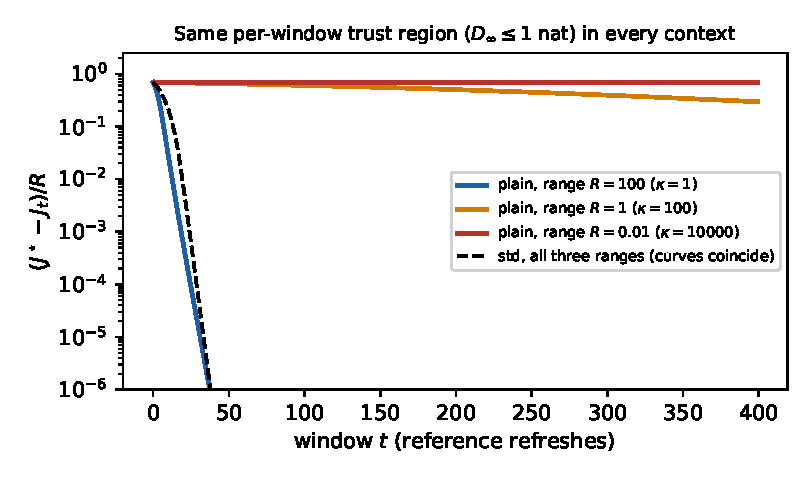
\includegraphics[width=0.66\textwidth]{figures/separation.pdf}
\caption{Relative suboptimality across windows (exact windows, tabular, $|\cY|=6$,
$G=16$) for three contexts whose rewards have the same shape but ranges $10^2$, $1$
and $10^{-2}$. Both algorithms get the same per-window trust region
$\Dinf(\pi_{t+1}\|\pi_t)\le1$ nat in every context (plain: $\beta=R_{\max}$; std:
$\beta=2\sqrt G$). The three std curves coincide exactly (Corollary~\ref{cor:invariance});
plain \rr{} slows down by the scale ratio $\kappa$ (Proposition~\ref{prop:separation}).}
\label{fig:separation}
\end{figure}

Finally, the agnostic analogue of REBEL's Theorem~1. Groups are drawn from
$\nu_t=\frac12(\pi_t+\mu)$ for a fixed full-support base distribution $\mu$, and the
standardizer is $\sigma_t(x)=\mathrm{std}_{\nu_t}\,r(x,\cdot)$. Let
$f_t=\beta\ln(\pi_{t+1}/\pi_t)$.

\begin{assumption}[Regression generalization, in standardized units]\label{ass:reg}
For all $t$,
$\E_x\E_{y,y'\sim\nu_t}\bigl(f_t(x,y)-f_t(x,y')-\frac{r(x,y)-r(x,y')}{\sigma_t(x)}\bigr)^2\le\varepsilon$.
\end{assumption}

\begin{theorem}[Agnostic regret bound]\label{thm:agnostic}
Let $\Delta_t=f_t-r/\sigma_t$, $\bar\Delta_t(x)=\E_{\nu_t}\Delta_t$,
$g_t=r/\sigma_t+\Delta_t-\bar\Delta_t$ and $A_t=g_t-\E_{\pi_t}g_t$, and assume
$|A_t|\le A$. Under Assumption~\ref{ass:reg}, with uniform $\pi_0$ and
$\beta=A\sqrt{T/\ln|\cY|}$ (for $T\ge\ln|\cY|$), every comparator $\pi^\star$ satisfies
\[
  \frac1T\sum_{t<T}\E_x\Bigl[\frac{J_{\pi^\star}(x)-J_t(x)}{\sigma_t(x)}\Bigr]
  \le2A\sqrt{\frac{\ln|\cY|}{T}}+\sqrt{6\,C_{\mu\to\pi^\star}\,\varepsilon},
  \qquad C_{\mu\to\pi^\star}=\max_{x,y}\frac{\pi^\star(y\mid x)}{\mu(y\mid x)}.
\]
If $\pi^\star$ is optimal in every context, then, since $\sigma_t\le R/2$,
$\frac1T\sum_t\E_x\bigl[(J^\star-J_t)/R(x)\bigr]\le A\sqrt{\ln|\cY|/T}+\sqrt{3C\varepsilon/2}$.
\end{theorem}

Every quantity here is measured in each context's own units:
\begin{itemize}[itemsep=1pt,topsep=2pt]
\item $\varepsilon$ is standardized, so a regressor cannot meet Assumption~\ref{ass:reg}
by fitting the large-scale contexts and ignoring the rest.
\item $A=O(1)$. The mixture keeps the standardizer away from zero,
$\sigma_t\ge\sigma_\mu/\sqrt2$, so the true standardized advantage is bounded by
$\sqrt2R/\sigma_\mu$, a ratio of scales. This is a second role for $\mu$, beyond
coverage.
\item The left side weights each context by $1/\sigma_t(x)$.
\end{itemize}
REBEL's bound is instead on $\E_x[J^\star-J_t]$ in raw units, with $A\sim R_{\max}$ and a
raw $\varepsilon$ dominated by the large-scale contexts; turning it into per-context
relative accuracy costs the scale ratio.

%------------------------------------------------------------------------------
\section{What standardization does to the Lagrangian reward}\label{sec:lagrangian}

\begin{proposition}[Branch-wise $\lambda$-invariance]\label{prop:branch}
Consider the reward~\eqref{eq:lagrangian}. If every member of a group is surely
infeasible ($\Pr_o[s_2\ge\tau]=0$ for each), then $r_i=\lambda(\E s_2-\tau)$ is an
increasing affine function of $\E s_2$. So the std targets coincide with those of
the pure content objective $\E s_2$, for every $\lambda>0$. If every member is surely
feasible, they coincide with those of $\E s_1$. The multiplier therefore matters only
for groups that straddle the floor. Under plain \rr{}, surely-infeasible groups get
targets scaled by $\lambda$ and a per-window KL scaled by $\lambda^2$. At $\lambda=0.01$ that is
about $10^{-4}$ of the budget of a feasible group whose scores spread comparably.
\end{proposition}

This is the benchmark-specific reason std works. At high $\tau$ the early policy is
mostly infeasible. Plain \rr{} then receives almost no signal, while \rrs{} receives
a full-budget update towards more content. Once groups are feasible, std gives a
full-budget update towards more sentiment. Groups straddling the floor rank
feasible members, spread by sentiment, above infeasible ones, which are compressed
together. The result is an automatic ``feasibility first, then objective''
curriculum, independent of $\lambda$.

\begin{proposition}[Monotone improvement in the stochastic order]\label{prop:monotone}
In the setting of Section~\ref{sec:rate}, $\pi_{t+1}(y)/\pi_t(y)\propto e^{\eta\zeta_t(y)}$
is nondecreasing in $r(y)$. So the law of $r$ under $\pi_{t+1}$ dominates that under
$\pi_t$ in the likelihood-ratio order, hence first-order stochastically:
$\E_{\pi_{t+1}}\phi(r)\ge\E_{\pi_t}\phi(r)$ for every nondecreasing $\phi$~\cite{shaked}. In
particular $J_{t+1}\ge J_t$ and $\Pr_{\pi_{t+1}}(r\ge a)\ge\Pr_{\pi_t}(r\ge a)$ for all
$a$. The squashing of Theorem~\ref{thm:finiteG} costs nothing here.
\end{proposition}

\begin{proposition}[A reliability-weighted trust region]\label{prop:reliability}
Let the observed rewards be $\hat r=r+\epsilon$, with $\E[\epsilon\mid y]=0$,
$\Var(\epsilon\mid y)=v(y)$, and noise independent across members. In the large-$G$
limit $\hat\sigma^2\to\sigma_{\mathrm{tot}}^2=\Var_q(r)+\E_qv$. The std target (for
$\ell_2$, or any even convex $\ell$ when $\epsilon-\epsilon'$ is symmetric) is
$\pi\propto\pref e^{r/(\beta\sigma_{\mathrm{tot}})}$, and with $q=\pref$
\[
  \KL(\pi\,\|\,\pref)=\frac{\varrho^2}{2\beta^2}+O(\beta^{-3}),\qquad
  \varrho^2=\frac{\Var_q(r)}{\Var_q(r)+\E_qv}\in[0,1].
\]
The quantity $\varrho^2$ is the reliability of the reward. Plain \rr{} moves
$\Var_q(r)/(2\beta^2)$ regardless of the noise. For a Monte Carlo reward averaged
over $n$ task-model samples, $v=v_1/n$, so the budget grows with $n$: std moves the
policy only as far as the reward can tell outputs apart.
\end{proposition}

\begin{remark}[The ``difficulty bias'' of std is the balancing we want]\label{rem:drgrpo}
Liu et al.~\cite{drgrpo} observe that GRPO's division by the in-group standard
deviation reweights prompts by $1/\sigma$, and they remove it in order to optimize
the average raw reward. In the multi-objective problem this reweighting is exactly
what equalizes the learning signal across $\tau$ (Propositions~\ref{prop:budget},
\ref{prop:balance} and~\ref{prop:gn}, Theorem~\ref{thm:rate}). Std optimizes the
scale-free objective $\E_x[(J^\star-J)/\mathrm{scale}(x)]$, which is what uniform
controllability asks for. Whether the reweighting is a bias depends on which of the
two objectives is intended.
\end{remark}

%------------------------------------------------------------------------------
\section{Directions to pursue}\label{sec:directions}

\begin{enumerate}[itemsep=2pt,topsep=2pt]
\item \emph{An M-estimation version of the agnostic theory.} Replace
Assumption~\ref{ass:reg} by an $\ell_1$/Huber excess-risk condition with finite-$G$
targets, and ask which $d$ gives the smallest error on heavy-tailed standardized
targets. REBEL leaves open whether losses other than the square loss help. Reward-side
clipping (Proposition~\ref{prop:softclip}) together with residual-side robustness
(Proposition~\ref{prop:symm}) is a concrete route to an answer.
\item \emph{Group size as a design knob.} $G$ sets the clip level $\approx\sqrt G$, the
largest late-phase step $\sqrt G/\beta$, and the position between ordinal and
cardinal learning. Holding the late-phase step fixed while changing $G$ calls for
$\beta\propto\sqrt G$.
\item \emph{Choose $\beta$ from a KL budget.} The per-window KL is $\approx1/(2\beta^2)$,
so $\beta=1/\sqrt{2\varepsilon_{\mathrm{target}}}$. For example, $\beta=\tfrac12$
corresponds to about $2$ nats per window (exactly $2$ for Gaussian-shaped rewards),
with finite-$G$ worst case $2\sqrt G/\beta$.
\item \emph{Decouple exploration from the step size.} Compute $\hat\sigma$ over the
on-policy members only, or under $\pref$, so that exploration affects coverage but not
the temperature (Remark~\ref{rem:sampler}). A small off-policy component still
floors the standardizer (Theorem~\ref{thm:agnostic}).
\item \emph{Comparative feedback.} By Proposition~\ref{prop:G2}, \rrs{} can run
directly on pairwise judgments (for instance from LLM judges), with REBEL's
minimax-winner guarantee (its Theorem~2). This matters when the scorers are
comparative rather than cardinal.
\item \emph{Explicit clipping.} Replace the implicit clip at $\approx\sqrt G$ by
$\mathrm{clip}(z,-c,c)$, which decouples robustness from group size.
\item \emph{Within-window dynamics.} Analyse the Adam steps with an on-policy sampler
as a semi-gradient flow towards the self-consistent fixed point of
Proposition~\ref{prop:fp}, including its dependence on the number of steps per window.
\item \emph{Several constraints.} Extend the branch-wise analysis to rewards with
several multipliers $\lambda_k$ and ask which regions of the constraint space make
each $\lambda_k$ irrelevant.
\end{enumerate}

\section{What the theory does not cover}\label{sec:limits}
The results are about idealized quantities. Windows are assumed solved exactly;
Theorem~\ref{thm:finiteG} and Section~\ref{sec:rate} use tabular policies, and
Theorem~\ref{thm:finiteG} is proved only for $\ell_2$. For $\ell_1$ and Huber we
checked numerically that the finite-$G$ minimizer is also rank-preserving and
inside the $2\sqrt G/\beta$ trust region (Appendix~\ref{app:checks}), but we have no
closed form. The implementation's sampler drifts within a window, which is only
partly captured by Propositions~\ref{prop:nofp}--\ref{prop:fp}. Finally, the theory
is about maximizing the constrained reward. Because the floor in~\eqref{eq:lagrangian}
is applied per task-model sample, that reward is a surrogate for a chance
constraint, not for $\E[s_2]\ge\tau$.

%==============================================================================
\appendix
\section{Proofs}\label{app:proofs}

\paragraph{Theorem~\ref{thm:target}.} If $\pi=\pi^\star_{\mathrm{std}}$ then
$h_\pi(x,y)=r(x,y)/\sigma_q(x)-\beta\log Z(x)$, so every residual vanishes and
$\cL^\infty=0\le\cL^\infty(\pi')$ for all $\pi'$. Conversely, $\cL^\infty(\pi)=0$ forces
$h_\pi(x,y)-h_\pi(x,y')=(r(x,y)-r(x,y'))/\sigma_q(x)$ for $q\otimes q$-almost every pair.
With full support this holds for all pairs, so $h_\pi(x,\cdot)-r(x,\cdot)/\sigma_q(x)$ is
constant in $y$, which is~\eqref{eq:target}. The variational form is the Gibbs
principle: with $\pi^\star_T\propto\pref e^{r/T}$ and normalizer $Z_T$,
$\E_\pi[r]-T\,\KL(\pi\|\pref)=T\log Z_T-T\,\KL(\pi\|\pi^\star_T)$, which is maximized at
$\pi=\pi^\star_T$; apply it with $T=\beta\sigma_q(x)$ in each context. \qed

\paragraph{Corollary~\ref{cor:invariance}.} $r_i\mapsto a r_i+b$ maps $\bar r\mapsto
a\bar r+b$ and $\hat\sigma\mapsto a\hat\sigma$, so $z_i$ is unchanged. \qed

\paragraph{Proposition~\ref{prop:budget}.} Write $t=1/\beta$. Then
$\log(\pi^\star/\pref)=tu-\Lambda(t)$ and $\E_{\pi^\star}u=\Lambda'(t)$, so
$\KL=t\Lambda'(t)-\Lambda(t)$ and the gain is $\sigma(\Lambda'(t)-\E_{\pref}u)=\sigma\Lambda'(t)$.
With $\Lambda(t)=\frac{t^2}{2}+\frac{\gamma t^3}{6}+O(t^4)$ one gets
$\KL=\frac{t^2}{2}+\frac{\gamma t^3}{3}+O(t^4)$; for a Gaussian $u$, $\Lambda=t^2/2$ exactly.
For (iii), if $\KL(\pi\|\pref)\le\varepsilon_\beta$, optimality of $\pi^\star$ for the
penalized objective gives
$\E_\pi r\le\E_{\pi^\star}r-\beta\sigma\bigl(\varepsilon_\beta-\KL(\pi\|\pref)\bigr)\le\E_{\pi^\star}r$.
Part (iv) is the same computation with $t=\sigma/\beta$. \qed

\paragraph{Proposition~\ref{prop:npg}.} Equation~\eqref{eq:md} is Theorem~\ref{thm:target}
with $\pref=q=\pi_t$. In logits, $\pi_t e^{\eta r}$ corresponds to $\theta_t+\eta r$, which
equals $\theta_t+\eta A_t$ up to a constant per context. With
$F=\mathrm{diag}(\pi)-\pi\pi^\top$ and $\nabla_\theta J=\pi\odot A$, we have $FA=\pi\odot A$
(because $\pi^\top A=0$), so $A$ is a natural gradient, and
$A^\top FA=\sum_y\pi A^2-(\pi^\top A)^2=\sigma^2$. \qed

\paragraph{Theorem~\ref{thm:finiteG}.} Write $e_i=h(y_i)-z_i$. Then
$\sum_{i<j}(e_i-e_j)^2=G\sum_ie_i^2-(\sum_ie_i)^2$, and $\sum_je_j=\sum_jh(y_j)$ because
$\sum_jz_j=0$. The derivative of the expected loss in $h(y)$ is
$2\,\E\bigl[\sum_i\1\{y_i=y\}\bigl(Gh(y)-Gz_i-\sum_jh(y_j)\bigr)\bigr]$. By
exchangeability this equals
$2G\,q(y)\bigl[(G-1)h(y)-G\zeta_q(y)-(G-1)\E_qh\bigr]$, which vanishes if and only if
$h(y)=\E_qh+\frac{G}{G-1}\zeta_q(y)$; this is consistent, since $\E_q\zeta_q=\E z_1=0$. The
loss is a convex quadratic in $h$ whose Hessian form
$\E[G\sum_i(h(y_i)-\bar h)^2]$ vanishes only for constant $h$ (full support, $G\ge2$), so
the minimizer is unique up to the constant absorbed by normalization. Pairs with
$y_i=y_j$ do not involve $h$ and do not affect the minimizer. \qed

\paragraph{Lemma~\ref{lem:phi}.} With $t=r-m'$ the group mean is $m'+t/G$, so
$r-\bar r=ct$. The within-group sum of squares decomposes as
$V'+c^2t^2+(G-1)(t/G)^2=V'+ct^2$. Divide by $G-1$ and take the square root. The
derivative and the limits follow directly. \qed

\paragraph{Corollary~\ref{cor:finiteG}.} (a)~$\zeta_q(y)=\E_{\mathrm{others}}[\varphi(r(y);\mathrm{others})]$
and the others do not depend on $y$, so Lemma~\ref{lem:phi} applies pointwise; in
flat configurations, $\sgn(r-v)$ is nondecreasing in $r$. (b)~By
Lemma~\ref{lem:bounded}, $|\zeta_q|\le\max_i|z_i|\le\frac{G-1}{\sqrt G}$, so
$|h-\E_qh|\le\frac{G}{G-1}\frac{G-1}{\sqrt G}=\sqrt G$. Because
$\pi^+$ and $\pref$ are both probability vectors, $\log(\pi^+/\pref)$ takes both signs, so
its maximum and minus its minimum are each at most the oscillation; hence both
$\Dinf$ and the KL are bounded by it. (c)~Saturation in Lemma~\ref{lem:phi}.
(d)~With probability $\to1$ all others equal $y^\star$. Then $\varphi(r^\star)=0$ (flat group)
and $\varphi(r(y))=-(G-1)/\sqrt G$, and bounded convergence gives the limit.
(e)~By the law of large numbers, $m'\to\E_qr$ and $V'/(G-1)\to\sigma_q^2$, so
$\varphi(r)\to(r-\E_qr)/\sigma_q$. \qed

\paragraph{Proposition~\ref{prop:nofp}.} With $\omega=\mathrm{logit}\,p$, the fixed-point
condition $h(\text{better})-h(\text{worse})=\Delta/\sigma_\pi$ reads
\[
  \beta\omega=\frac{1}{\sqrt{p(1-p)}}=2\cosh(\omega/2).
\]
Setting $s=\omega/2$, this is $\beta s=\cosh s$, which is solvable if and only if
$\beta\ge\min_s\cosh(s)/s$. The minimum is attained where $s\tanh s=1$
($s\approx1.200$, $\beta_c\approx1.5089$). When there is no solution,
$2\cosh(\omega/2)/\beta>\omega$ for all $\omega\ge0$, so the regression target always lies
above the current log-odds. \qed

\paragraph{Proposition~\ref{prop:fp}.} $\zeta_q(y)=\sum_mP_q(m)\,\varphi(r(y);m)$ over the
multisets $m$ of the other members, where $P_q(m)$ is a multinomial polynomial in
$q$. The map is therefore continuous from the simplex to itself, and Brouwer's
theorem gives a fixed point. Corollary~\ref{cor:finiteG}(b) holds for every $q$. \qed

\paragraph{Proposition~\ref{prop:firstorder}.} At $\pi=\pref$ the residual is
$-(z_i-z_j)$ and $\psi$ is odd, so
$\nabla\cL=-\frac{1}{SP}\sum_{i<j}\psi(z_i-z_j)(\nabla h_i-\nabla h_j)=-\frac{1}{SP}\sum_i\nabla h_i\,u_i$
with $\nabla h_i=\beta\nabla\log\pi(y_i)$. For $\ell_2$,
$u_i=2\sum_{j\neq i}(z_i-z_j)=2(Gz_i-\sum_jz_j)=2Gz_i$. For $\ell_1$, $u_i$ counts the members
below $y_i$ minus those above it. \qed

\paragraph{Proposition~\ref{prop:symm}.} In both cases $\epsilon_i-\epsilon_j$ and
$\epsilon_j-\epsilon_i$ have the same law. For even convex $\ell$, the function
$h\mapsto\E\,\ell(h-c-\xi)$ with $\xi$ symmetric is convex and even about $c$, so it
is minimized at $h=c$; uniqueness follows under the stated conditions. \qed

\paragraph{Lemma~\ref{lem:bounded}.} The vector $z$ is orthogonal to $\mathbf{1}$ and
$\|z\|^2=G-1$. For a unit vector $e_i$, the component of $e_i$ orthogonal to $\mathbf{1}$
has norm $\sqrt{(G-1)/G}$, so $|z_i|\le\sqrt{(G-1)/G}\,\sqrt{G-1}$. For
$w=e_i-e_j\perp\mathbf{1}$, $|z_i-z_j|\le\|w\|\,\|z\|=\sqrt{2(G-1)}$. Equality holds for
$z\parallel e_i-\mathbf{1}/G$ and for $z\parallel e_i-e_j$, respectively. \qed

\paragraph{Proposition~\ref{prop:balance}.} $\sum_{i<j}(x_i-x_j)^2=G\sum_i(x_i-\bar x)^2=G(G-1)\hat\sigma_x^2$;
divide by $G(G-1)/2$ pairs and use $\hat\sigma_z=1$. \qed

\paragraph{Corollary~\ref{cor:grpo}.} By Proposition~\ref{prop:firstorder} with $u_i=2Gz_i$ and $P=G(G-1)/2$,
\[
  \nabla\cL=-\frac{2\beta G}{SP}\sum z_i\nabla\log\pi(y_i)
  =\frac{4\beta G}{G-1}\cdot\Bigl(-\frac{1}{SG}\sum z_i\nabla\log\pi(y_i)\Bigr).\qquad\qed
\]

\paragraph{Proposition~\ref{prop:G2}.} For $G=2$, $\bar r=(r_1+r_2)/2$ and
$\hat\sigma=|r_1-r_2|/\sqrt2$, so $z_1-z_2=\sqrt2\sgn(r_1-r_2)$ and
$\zeta_q(y)=\E_{y'}\sgn(r(y)-r(y'))/\sqrt2=l_q(y)/\sqrt2$. Theorem~\ref{thm:finiteG} with
$G/(G-1)=2$ gives $h-\E h=\sqrt2\,l_q$. Part (i) is~\eqref{eq:loss} with these targets,
and (iii) holds because signs are invariant to increasing maps. If
$\epsilon,\epsilon'$ are i.i.d.\ Gumbel, $\epsilon-\epsilon'$ is logistic, so
$\Pr[\hat r>\hat r']$ is a logistic function of $r-r'$. \qed

\paragraph{Proposition~\ref{prop:softclip}.} Substitute $V'=(G-2)s_-^2$ in
Lemma~\ref{lem:phi}: $\varphi'(0)=\sqrt{G-1}\,c/\sqrt{V'}$, and the two terms under the root
balance at $ct^2=V'$. \qed

\paragraph{Proposition~\ref{prop:gn}.} Because $\E_\nu\tilde g=0$ and $\E_\nu u_c=0$ in each
context, and $y,y'$ are i.i.d., the linearized loss is
$\E\bigl(\beta(\tilde g-\tilde g')^\top\delta-(u_c-u_c')\bigr)^2=2\,\E_x\E_\nu\bigl(\beta\tilde g^\top\delta-u_c\bigr)^2$:
ordinary least squares of $u_c$ on the features $\beta\tilde g$. The normal equations give
$\beta^2F_\nu\delta=\beta\E[\tilde gu_c]=\beta\E[gu_c]$, whose minimum-norm solution
is~\eqref{eq:gn}. The fitted values $\beta\tilde g^\top\delta^\star$ are the orthogonal
projection $\Pi u_c$, so $\beta^2\delta^{\star\top}F_\nu\delta^\star=\|\Pi u_c\|^2\le\|u_c\|^2=\E_x\Var_\nu(u)=1$,
with equality if and only if $u_c$ lies in the span. With $\nu=\pi_t$, $F_\nu$ is the Fisher
information, and the second-order expansion of the KL gives the trust-region
statement. For plain \rr{}, replace $u_c$ by $r_c$, whose squared norm is
$\E_x\Var_\nu r=\E_x\sigma^2(x)\,\E_\nu u_c^2$. \qed

\paragraph{Proposition~\ref{prop:gnfinite}.} Using
$\sum_{i<j}(g_i-g_j)(g_i-g_j)^\top=G\hat C$ and
$\sum_{i<j}(g_i-g_j)(z_i-z_j)=G\sum_iz_i(g_i-\bar g)=G\sum_iz_ig_i$, the normal equations are
$\beta^2G\hat C\delta=\beta G\sum z_ig_i$. If the centered scores have rank $G-1$, the system
$\beta(g_i-\bar g)^\top\delta=z_i$ is consistent: both sides satisfy the one linear
relation $\sum_i(\cdot)=0$. The least-squares solution therefore has zero residual,
and $\Delta_i-\bar\Delta=z_i$. \qed

\paragraph{Corollary~\ref{cor:trpo}.} The TRPO step is
$\Delta=\sqrt{2\delta_{\mathrm{TR}}/(b^\top F^\dagger b)}\,F^\dagger b$ with $b=\nabla J$.
In the tabular case $F^\dagger b=A$ (up to constants) and $b^\top F^\dagger b=\sigma^2$, so
$\Delta=\sqrt{2\delta_{\mathrm{TR}}}\,A/\sigma$, which equals $A/(\beta\sigma)$ exactly when
$\delta_{\mathrm{TR}}=1/(2\beta^2)$. For a single context in a general parameterization,
$\delta^\star$ has TRPO's direction $F^\dagger\E[gu_c]$, and its quadratic length is
$R^2_{\mathrm{compat}}/\beta^2$ by~\eqref{eq:gnbound}. \qed

\paragraph{Lemma~\ref{lem:zeta}.} (i)~$\E_q\zeta_q=\E z_1=\frac1G\E\sum_iz_i=0$.
(ii)~Lemma~\ref{lem:bounded}. (iii)~By Jensen,
$\E_q\zeta_q^2\le\E z_1^2=\frac1G\E\sum_iz_i^2\le\frac{G-1}{G}$. (iv)~For $y_1=y^\star$,
$r^\star-m'\ge0$. By Popoviciu's inequality the group's sample variance is at most
$\frac{G}{G-1}\frac{R^2}{4}$, so
$z_1=c(r^\star-m')/\hat\sigma\ge\frac{2}{R}\bigl(\frac{G-1}{G}\bigr)^{3/2}(r^\star-m')$. This also
holds when $\hat\sigma=0$, since then $r^\star=m'$. Take expectations and use
$\E m'=\E_qr$. \qed

\paragraph{Theorem~\ref{thm:global}.} (i)~is Proposition~\ref{prop:monotone} applied to
the threshold $a=J^\star$. (ii)~The increment is $\eta(\zeta_t(y^\star)-\zeta_t(y))$ and
$\zeta_t(y^\star)-\zeta_t(y)=\E_{\mathrm{others}}[\varphi(r^\star)-\varphi(r(y))]$. Every
configuration contributes $\ge0$ by Corollary~\ref{cor:finiteG}(a). The configurations in
which all others lie in $\cY^\star$ have probability $\pi_t(\cY^\star)^{G-1}$ and contribute
$0-(-(G-1)/\sqrt G)$. Multiplying by $\eta=G/((G-1)\beta)$ gives the bound; use (i) for the
second inequality. \qed

\paragraph{Theorem~\ref{thm:rate}.} \emph{Mirror-descent inequality with local norms.} Let
$\pi_{t+1}=\pi_te^{\eta\zeta_t}/Z_t$. For any comparator $p$,
$\KL(p\|\pi_{t+1})-\KL(p\|\pi_t)=-\eta\E_p\zeta_t+\log Z_t$. Since $e^a\le1+a+a^2$ for
$a\le1$ and $\eta\zeta_t\le\eta\frac{G-1}{\sqrt G}=\frac{\sqrt G}{\beta}\le1$,
$\log Z_t\le\log(1+\eta\E_{\pi_t}\zeta_t+\eta^2\E_{\pi_t}\zeta_t^2)\le\eta^2\frac{G-1}{G}$,
using Lemma~\ref{lem:zeta}(i),(iii). Summing,
$\sum_t\E_p\zeta_t\le\KL(p\|\pi_0)/\eta+\eta T\frac{G-1}{G}$. Take $p=\delta_{y^\star}$, so
$\KL=\ln|\cY|$, apply Lemma~\ref{lem:zeta}(iv), and substitute $\eta$. The tuned $\beta$
minimizes $a\beta+1/\beta$ with $a=(G-1)\ln|\cY|/(GT)$, giving
$2\sqrt a/\kappa_G=\frac{G}{G-1}\sqrt{\ln|\cY|/T}$. \qed

\paragraph{Proposition~\ref{prop:separation}.} (i)~The same inequality with $\eta=1/\beta$,
$A_t=r-J_t$, $|A_t|\le R(x)$ and $\E_{\pi_t}A_t^2\le R(x)^2/4$ (Popoviciu). The condition
$\eta|A_t|\le1$ in every context requires $\beta\ge R_{\max}$. Substituting the stated
$\beta$ gives the expression. (ii)~Plain: $\osc\log(\pi_{t+1}/\pi_t)=R(x)/\beta\le R_{\max}/\beta$.
Std: Corollary~\ref{cor:finiteG}(b). In the binary case the plain gain is
$R(x)/\beta=B/\kappa(x)$. The std gain is
$\frac{G}{G-1}(\zeta_q(\mathrm{better})-\zeta_q(\mathrm{worse}))/\beta$, which is an average
of in-group gaps $D(k)=\sqrt{G(G-1)/(k(G-k))}\ge2\sqrt{(G-1)/G}$ over the number $k$ of better
members, with weights summing to $(G-1)/G$ before the factor $G/(G-1)$. Relative
suboptimality after log-odds $L$ is $1/(1+e^{L})$. \qed

\paragraph{Theorem~\ref{thm:agnostic}.} This is REBEL's proof of its Theorem~1 applied to
the iteration-dependent reward $r_t=r/\sigma_t$. That argument never uses that the
reward is the same at every iteration (its Appendix~E runs it with iteration-dependent
rewards). We record the steps.
(1)~For $y,y'$ i.i.d.\ from $\nu_t$,
$\E(\Delta_t(y)-\Delta_t(y'))^2=2\E_{\nu_t}(\Delta_t-\bar\Delta_t)^2$, so
$\E_x\E_{\nu_t}(\Delta_t-\bar\Delta_t)^2\le\varepsilon/2$. Since $\pi_t\le2\nu_t$ and $\mu\le2\nu_t$,
the same quantity under $\pi_t$ or $\mu$ is at most $\varepsilon$.
(2)~$\pi_{t+1}\propto\pi_te^{f_t/\beta}\propto\pi_te^{A_t/\beta}$, with $|A_t|/\beta\le1$ and
$\E_{\pi_t}A_t=0$. The local-norm inequality above gives
$\sum_t\E_{\pi^\star}A_t\le\beta\ln|\cY|+TA^2/\beta=2A\sqrt{T\ln|\cY|}$ in every context.
(3)~$J_{\pi^\star}-J_t=\sigma_t\,\E_{\pi^\star}A_t^\star$ with $A_t^\star=r_t-\E_{\pi_t}r_t$, and
$A_t^\star-A_t=-(\Delta_t-\bar\Delta_t)+\E_{\pi_t}(\Delta_t-\bar\Delta_t)$. Hence
$\E_{\nu_t}(A^\star_t-A_t)^2\le2\E_{\nu_t}(\Delta_t-\bar\Delta_t)^2+2\E_{\pi_t}(\Delta_t-\bar\Delta_t)^2\le6\E_{\nu_t}(\Delta_t-\bar\Delta_t)^2$,
whose context average is at most $3\varepsilon$. By Cauchy--Schwarz and
$\pi^\star\le C_{\nu_t\to\pi^\star}\nu_t$ with $C_{\nu_t\to\pi^\star}\le2C_{\mu\to\pi^\star}$,
$\E_x\E_{\pi^\star}(A_t^\star-A_t)\le\sqrt{6C_{\mu\to\pi^\star}\varepsilon}$.
(4)~Average (2) and (3) over $x$ and $t$. For the corollary, $J^\star-J_t\ge0$ and
$\sigma_t\le R/2$ (Popoviciu). Finally,
$\Var_{\nu_t}r\ge\frac12\Var_\mu r$ by the law of total variance, which gives
$\sigma_t\ge\sigma_\mu/\sqrt2$. \qed

\paragraph{Proposition~\ref{prop:branch}.} Corollary~\ref{cor:invariance} with
$a=\lambda$ and $b=-\lambda\tau$ (infeasible), or with $a=1$ and $b=0$ (feasible). For plain
\rr{} the targets scale by $\lambda$, and Proposition~\ref{prop:budget}(iv) gives the KL. \qed

\paragraph{Proposition~\ref{prop:monotone}.} Let $w=e^{\eta\zeta_t}$, nondecreasing in $r$
by Corollary~\ref{cor:finiteG}(a). For any $a$, both $\1\{r\ge a\}$ and $w$ are
nondecreasing in $r$, so by Chebyshev's (Harris') inequality
$\E_{\pi_t}[\1\{r\ge a\}w]\ge\E_{\pi_t}[\1\{r\ge a\}]\,\E_{\pi_t}[w]$, i.e.\
$\Pr_{\pi_{t+1}}(r\ge a)\ge\Pr_{\pi_t}(r\ge a)$. This is first-order stochastic dominance. \qed

\paragraph{Proposition~\ref{prop:reliability}.} By the law of total variance,
$\Var(\hat r)=\Var_q(r)+\E_qv$. The pairwise target
$(\hat r-\hat r')/\sigma_{\mathrm{tot}}$ has conditional mean (and, under symmetric noise,
conditional median) $(r-r')/\sigma_{\mathrm{tot}}$. This difference is realizable, so it is the
minimizer (Proposition~\ref{prop:symm}). The KL of an exponential tilt by $t\,r$ is
$\frac{t^2}{2}\Var_q(r)+O(t^3)$; take $t=1/(\beta\sigma_{\mathrm{tot}})$. \qed

\section{Numerical checks}\label{app:checks}
The script \texttt{checks.py} (next to this file; numpy only, no repository code)
verifies the quantitative claims on small tabular problems. The agnostic bound
(Theorem~\ref{thm:agnostic}) is a reduction to REBEL's proof and is not simulated. Where possible it
enumerates groups exactly, using multisets of the $G-1$ other members, which makes
$\zeta_q$ exact up to $G=16$. All checks pass. The main ones:
\begin{center}\small
\begin{tabularx}{\textwidth}{@{}>{\raggedright\arraybackslash}X>{\raggedright\arraybackslash}p{6.2cm}@{}}
\toprule
claim & result \\
\midrule
Thm.~\ref{thm:finiteG}: $\ell_2$ minimizer $=\frac{G}{G-1}\zeta_q$ (brute force, $G=2,\dots,5$) & max error $2\times10^{-15}$\\
Prop.~\ref{prop:G2}: $G=2$ target $=\sqrt2\,l_q$ & error $2\times10^{-16}$\\
Lemma~\ref{lem:phi} formula; Samuelson and pair bounds (tight) & relative error $4\times10^{-16}$\\
Cor.~\ref{cor:finiteG}(a),(b) at $G=16$ (40 random samplers) & rank-preserving; oscillation $\le0.90\times$ bound\\
Cor.~\ref{cor:finiteG}(d): late-phase gain & $\to\sqrt G$ for $G=2,4,16,64$\\
Binary gain range, Fig.~\ref{fig:squashing}(b) & $[\sqrt2,\sqrt G]$; $m_G=1.414, 1.732, 1.866, 1.984, 1.998$ ($G=2,3,4,8,16$)\\
Prop.~\ref{prop:nofp}: threshold $\beta_c$ & $1.50888$\\
Prop.~\ref{prop:fp}: finite-$G$ fixed point ($G=16$, $\beta=\frac12$) & log-odds $7.99\le16$\\
Prop.~\ref{prop:budget}: CGF identities; Gaussian KL; scale invariance & exact; $2.000000$; std KL constant over 6 decades, plain KL $2\times10^{-6}$ to $5.1$\\
Prop.~\ref{prop:npg}, Cor.~\ref{cor:trpo}: Fisher norm; TRPO $=$ std window & exact\\
Prop.~\ref{prop:balance}: window-start loss $=2$ per non-flat group & exact\\
Prop.~\ref{prop:gn}: $\beta^2\delta^\top F\delta=R^2_{\mathrm{compat}}$ & $0.20$, $0.44$, $1.00$ for feature dimension $4$, $12$, $29$ of $29$\\
Prop.~\ref{prop:gnfinite}: interpolation, unit in-group spread & exact\\
Lemma~\ref{lem:zeta}(iii),(iv) at $G=16$ & hold; (iv) tight to a factor $0.89$\\
Thm.~\ref{thm:global}: monotone $\pi_t(\cY^\star)$; increment bound & holds\\
Thm.~\ref{thm:rate} ($G=16$, $|\cY|=6$, $T=3000$, ranges $10^{-2},1,10^2$) & std $0.0047$ in every context (bound $0.0261$); plain $0.44$, $0.37$, $0.012$\\
Prop.~\ref{prop:reliability}: KL vs.\ $\varrho^2/(2\beta^2)$ & within $1\%$ for $\varrho^2\in[0.1,1]$\\
Prop.~\ref{prop:monotone}; Prop.~\ref{prop:branch} & hold; exact\\
$\ell_1$ and Huber finite-$G$ minimizers (IRLS, $G=4$) & rank-preserving; oscillation $\le0.85\times$ bound\\
\bottomrule
\end{tabularx}
\end{center}

\begin{thebibliography}{99}\small
\bibitem{draft} A.~Deshmukh and L.~Varshney. \emph{Multi Objective Optimization in LLMs}. Draft.
\bibitem{slides} A.~Deshmukh. \emph{Multi-Objective Prompt Optimization in LLMs}. Talk slides (LLNL).
\bibitem{rebel} Z.~Gao, J.~D.~Chang, W.~Zhan, O.~Oertell, G.~Swamy, K.~Brantley, T.~Joachims, J.~A.~Bagnell, J.~D.~Lee, W.~Sun. REBEL: Reinforcement learning via regressing relative rewards. \emph{NeurIPS}, 2024.
\bibitem{ipo} M.~G.~Azar, M.~Rowland, B.~Piot, D.~Guo, D.~Calandriello, M.~Valko, R.~Munos. A general theoretical paradigm to understand learning from human preferences. \emph{AISTATS}, 2024.
\bibitem{spo} G.~Swamy, C.~Dann, R.~Kidambi, Z.~S.~Wu, A.~Agarwal. A minimaximalist approach to reinforcement learning from human feedback. \emph{ICML}, 2024.
\bibitem{kakade} S.~M.~Kakade. A natural policy gradient. \emph{NeurIPS}, 2001.
\bibitem{trpo} J.~Schulman, S.~Levine, P.~Abbeel, M.~Jordan, P.~Moritz. Trust region policy optimization. \emph{ICML}, 2015.
\bibitem{sutton} R.~S.~Sutton, D.~McAllester, S.~Singh, Y.~Mansour. Policy gradient methods for reinforcement learning with function approximation. \emph{NeurIPS}, 1999.
\bibitem{beck} A.~Beck and M.~Teboulle. Mirror descent and nonlinear projected subgradient methods for convex optimization. \emph{Operations Research Letters}, 31(3), 2003.
\bibitem{huber} P.~J.~Huber. Robust estimation of a location parameter. \emph{Annals of Mathematical Statistics}, 35(1), 1964.
\bibitem{samuelson} P.~A.~Samuelson. How deviant can you be? \emph{Journal of the American Statistical Association}, 63(324), 1968.
\bibitem{nes} D.~Wierstra, T.~Schaul, T.~Glasmachers, Y.~Sun, J.~Peters, J.~Schmidhuber. Natural evolution strategies. \emph{JMLR}, 15, 2014.
\bibitem{ziegler} D.~M.~Ziegler, N.~Stiennon, J.~Wu, T.~B.~Brown, A.~Radford, D.~Amodei, P.~Christiano, G.~Irving. Fine-tuning language models from human preferences. arXiv:1909.08593, 2019.
\bibitem{drgrpo} Z.~Liu et al. Understanding R1-Zero-like training: A critical perspective. arXiv:2503.20783, 2025.
\bibitem{shaked} M.~Shaked and J.~G.~Shanthikumar. \emph{Stochastic Orders}. Springer, 2007.
\end{thebibliography}

\end{document}
